\documentclass[12pt]{article}
\usepackage{graphicx}
\usepackage{float}
\usepackage{amsmath}
\usepackage{amscd}
\usepackage{hyperref}
\usepackage{enumerate}
\usepackage{amsfonts}
\usepackage{amssymb}
\usepackage[utf8]{inputenc}
\usepackage{amsthm}
\usepackage{subcaption}
\usepackage{listings}
\usepackage{tikz}
\usepackage{color} %red, green, blue, yellow, cyan, magenta, black, white
\usepackage{fullpage}
\usepackage{mathtools}
\usepackage{booktabs}
\usepackage{longtable}

\definecolor{mygreen}{RGB}{28,172,0} % color values Red, Green, Blue
\definecolor{mylilas}{RGB}{170,55,241}

\newtheorem{theorem}{Teorema}
\newtheorem{lem}[theorem]{Lemma}
\newtheorem{dfn}{Definición}
\newtheorem{cor}[theorem]{Corolario}
\newtheorem{obs}{Obs}
\newtheorem{rem}{Remark}
\newtheorem{prob}{Problema}

\newcommand*\circled[1]{\tikz[baseline=(char.base)]{
            \node[shape=circle,draw,inner sep=.05pt] (char) {#1};}}
            


\newtheoremstyle{named}{}{}{\itshape}{}{\bfseries}{.}{.5em} {\thmnote{#3 }#1}
\theoremstyle{named}
\newtheorem*{namedtheorem}{}



\newcounter{exercisecounter}
\newenvironment{ex}{\begin{quote}%
    \refstepcounter{exercisecounter}%
  \textbf{Ejercicio \arabic{exercisecounter}}%
  \quad
}{%
\end{quote}%
}
\newcounter{ejemplocounter}
\newenvironment{ej}{\begin{quote}%
    \refstepcounter{ejemplocounter}%
  \textbf{Ejemplo \arabic{ejemplocounter}}%
  \quad
}{%
\end{quote}%
}

\renewcommand{\d}[1]{\ensuremath{\operatorname{d}\!{#1}}}

\DeclarePairedDelimiter{\ceil}{\lceil}{\rceil}


\newcommand{\folder}{./Effect}

\begin{document}


\title{Treatment effects}

\author{Instituto Tecnológico Autónomo de México}
\date{\today}
\maketitle


\hrulefill


\section{\Huge{Some Summary Statistics}}

\vspace{7mm}

\subsection*{Presence of actors}


\begin{center}
\scriptsize{
\begin{table}[htbp]\centering \caption{Presence of actors \label{sumstat}}
\begin{tabular}{l c c c c c}\hline\hline
\multicolumn{1}{c}{\textbf{Variable}} & \textbf{Mean}
 & \textbf{Std. Dev.}& \textbf{Min.} &  \textbf{Max.} & \textbf{N}\\ \hline
p\_actor & 0.151 & 0.358 & 0 & 1 & 2183\\
p\_ractor & 0.827 & 0.378 & 0 & 1 & 2183\\
p\_dem & 0.011 & 0.102 & 0 & 1 & 2183\\
p\_rdem & 0.44 & 0.496 & 0 & 1 & 2183\\
\hline\end{tabular}
\end{table}
}
\end{center}

We decompose who showed up in all the possible combinations; we use 1,2,3,4 subscripts to denote the different parties 1: Employee; 2: Employee’s Lawyer;  3: Firm; 4: Firm’s Lawyer. 


\begin{center}
\scriptsize{
\begin{table}[htbp]\centering \caption{Presence of actors \label{sumstat}}
\begin{tabular}{l c c c c c}\hline\hline
\multicolumn{1}{c}{\textbf{Variable}} & \textbf{Mean}
 & \textbf{Std. Dev.}& \textbf{Min.} &  \textbf{Max.} & \textbf{N}\\ \hline
v0 & 0.117 & 0.321 & 0 & 1 & 3114\\
v1 & 0.006 & 0.08 & 0 & 1 & 3114\\
v2 & 0.383 & 0.486 & 0 & 1 & 3114\\
v3 & 0.001 & 0.031 & 0 & 1 & 3114\\
v4 & 0.026 & 0.16 & 0 & 1 & 3114\\
v12 & 0.056 & 0.23 & 0 & 1 & 3114\\
v13 & 0 & 0.018 & 0 & 1 & 3114\\
v14 & 0.003 & 0.057 & 0 & 1 & 3114\\
v23 & 0.001 & 0.031 & 0 & 1 & 3114\\
v24 & 0.318 & 0.466 & 0 & 1 & 3114\\
v34 & 0 & 0.018 & 0 & 1 & 3114\\
v123 & 0 & 0 & 0 & 0 & 3114\\
v124 & 0.081 & 0.273 & 0 & 1 & 3114\\
v134 & 0 & 0.018 & 0 & 1 & 3114\\
v234 & 0.003 & 0.057 & 0 & 1 & 3114\\
v1234 & 0.003 & 0.054 & 0 & 1 & 3114\\
\hline\end{tabular}
\end{table}
}
\end{center}

\pagebreak

\subsection*{Summary statistics for survey variables}

\begin{center}
\scriptsize{
\begin{table}[htbp]\centering \caption{SS survey variables \label{sumstat}}
\begin{tabular}{l c c c c c}\hline\hline
\multicolumn{1}{c}{\textbf{Variable}} & \textbf{Mean}
 & \textbf{Std. Dev.}& \textbf{Min.} &  \textbf{Max.} & \textbf{N}\\ \hline
Initial prob employee & 79.812 & 24.906 & 10 & 100 & 223\\
Initial amount employee & 62736.224 & 87655.907 & 0 & 600000 & 188\\
Exit prob employee & 71.076 & 28.445 & 10 & 100 & 171\\
Exit amount employee & 54801.663 & 66298.621 & 0 & 350000 & 142\\
Initial prob employee's lawyer & 77.762 & 20.026 & 2 & 100 & 965\\
Initial amount employee's lawyer & 97572.459 & 112949.152 & 0 & 700000 & 768\\
Exit prob employee's lawyer & 67.505 & 24.514 & 1 & 100 & 733\\
Exit amount employee's lawyer & 87234.616 & 96300.243 & 0 & 600000 & 568\\
Initial prob firm's lawyer & 40.363 & 22.95 & 1 & 100 & 584\\
Initial amount firm's lawyer & 59030.199 & 82031.346 & 0 & 662451 & 462\\
Exit prob firm's lawyer & 42.416 & 23.352 & 1 & 100 & 440\\
Exit amount firm's lawyer & 56965.815 & 70131.048 & 0 & 480001 & 363\\
Buys goods & 0.074 & 0.263 & 0 & 1 & 229\\
Works & 0.426 & 0.496 & 0 & 1 & 230\\
Looking for a job & 0.551 & 0.498 & 0 & 1 & 225\\
\hline\end{tabular}
\end{table}
}
\end{center}


\begin{center}
\scriptsize{% Table generated by Excel2LaTeX from sheet 'TAB_survey'
\begin{tabular}{rr}
\toprule
\multicolumn{2}{c}{Anger employee} \\
\midrule
\midrule
\multicolumn{1}{l}{A lot} & 127 \\
\multicolumn{1}{l}{Fairly} & 37 \\
\multicolumn{1}{l}{Little } & 15 \\
\multicolumn{1}{l}{Nothing} & 34 \\
\midrule
\multicolumn{2}{c}{Education employee} \\
\midrule
\midrule
\multicolumn{1}{l}{Elementary} & 15 \\
\multicolumn{1}{l}{Secondary} & 58 \\
\multicolumn{1}{l}{High-School} & 61 \\
\multicolumn{1}{l}{+ High School} & 79 \\
\midrule
\multicolumn{2}{c}{Cases employee's lawyer} \\
\midrule
\midrule
\multicolumn{1}{l}{1-10} & 93 \\
\multicolumn{1}{l}{11-30} & 114 \\
\multicolumn{1}{l}{31-100} & 222 \\
\multicolumn{1}{l}{+ 100} & 441 \\
\midrule
\multicolumn{2}{c}{Cases firm's lawyer} \\
\midrule
\midrule
\multicolumn{1}{l}{1-10} & 41 \\
\multicolumn{1}{l}{11-30} & 48 \\
\multicolumn{1}{l}{31-100} & 115 \\
\multicolumn{1}{l}{+ 100} & 328 \\
\bottomrule
\end{tabular}%
}
\end{center}


\begin{center}
\scriptsize{% Table generated by Excel2LaTeX from sheet 'NA'
\begin{tabular}{rr}
\toprule
Variable & Missing values \\
\midrule
\multicolumn{2}{c}{Employee} \\
\midrule
\midrule
\multicolumn{1}{l}{Initial prob employee } & 13 \\
\multicolumn{1}{l}{Initial amount employee } & 45 \\
\multicolumn{1}{l}{Exit prob employee } & 56 \\
\multicolumn{1}{l}{Exit amount employee } & 83 \\
\multicolumn{1}{l}{Buys goods} & 6 \\
\multicolumn{1}{l}{Works} & 7 \\
\multicolumn{1}{l}{Looking for a job} & 12 \\
\multicolumn{1}{l}{Anger employee} & 0 \\
\multicolumn{1}{l}{Education employee} & 0 \\
\midrule
\multicolumn{2}{c}{Employee's Lawyer} \\
\midrule
\midrule
\multicolumn{1}{l}{Initial prob employee's lawyer} & 15 \\
\multicolumn{1}{l}{Initial amount employee's lawyer} & 188 \\
\multicolumn{1}{l}{Exit prob employee's lawyer} & 192 \\
\multicolumn{1}{l}{Exit amount employee's lawyer} & 339 \\
\multicolumn{1}{l}{Cases employee's lawyer} & 0 \\
\midrule
\multicolumn{2}{c}{Firm's Lawyer} \\
\midrule
\midrule
\multicolumn{1}{l}{Initial prob Firm's lawyer} & 10 \\
\multicolumn{1}{l}{Initial amount Firm's lawyer} & 113 \\
\multicolumn{1}{l}{Exit prob Firm's lawyer} & 126 \\
\multicolumn{1}{l}{Exit amount Firm's lawyer} & 189 \\
\multicolumn{1}{l}{Cases firm's lawyer} & 0 \\
\bottomrule
\end{tabular}%
}
\end{center}


\pagebreak

\subsection*{Update in beliefs}

The update in beliefs is measured in relative terms, this is the percentage deviation of the exit survey with respect to the entrance survey
\[\frac{exit-initial}{initial}\]

 We provide two measures: Update in beliefs in probability and payment.\\

\begin{center}
\scriptsize{
\begin{table}[htbp]\centering \caption{Update in beleifs \label{sumstat}}
\begin{tabular}{l c c c c c}\hline\hline
\multicolumn{1}{c}{\textbf{Variable}} & \textbf{Mean}
 & \textbf{Std. Dev.}& \textbf{Min.} &  \textbf{Max.} & \textbf{N}\\ \hline
update\_emp\_fir\_law & -0.026 & 1.171 & -1 & 9 & 180\\
update\_emp & -0.106 & 0.578 & -1 & 2.2 & 70\\
update\_emp\_law & -0.216 & 0.560 & -1 & 1.875 & 210\\
\hline\end{tabular}
\end{table}
}
\end{center}



\begin{figure}[H]
\label{diff}
\begin{center}
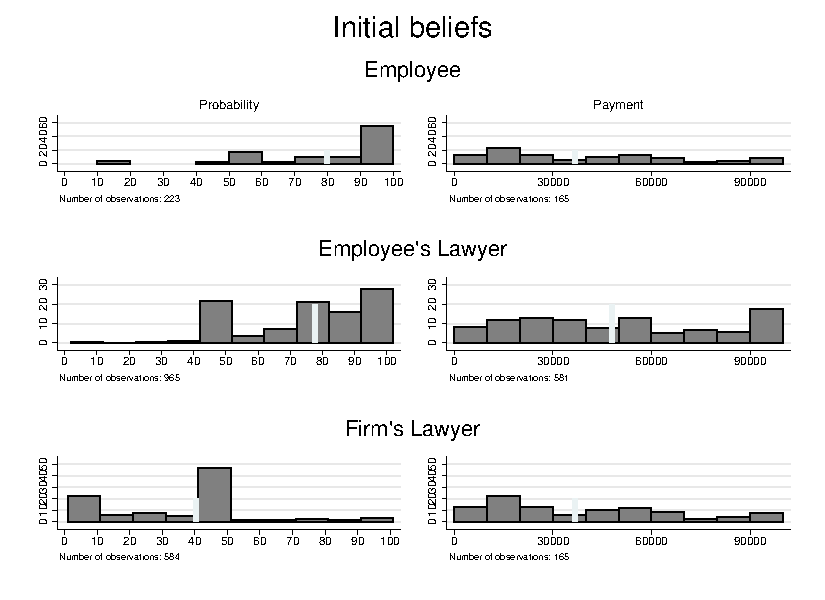
\includegraphics[width=\textwidth]{./Figures/belief.pdf}
\end{center}
{\footnotesize \textit{The histograms are trimmed at the 90 percentile in the case for amount. Width of bins are \$50,000 pesos for the case of amount and 10\% for the case of probability.}}
\end{figure}


\begin{figure}[H]
\label{update}
\begin{center}
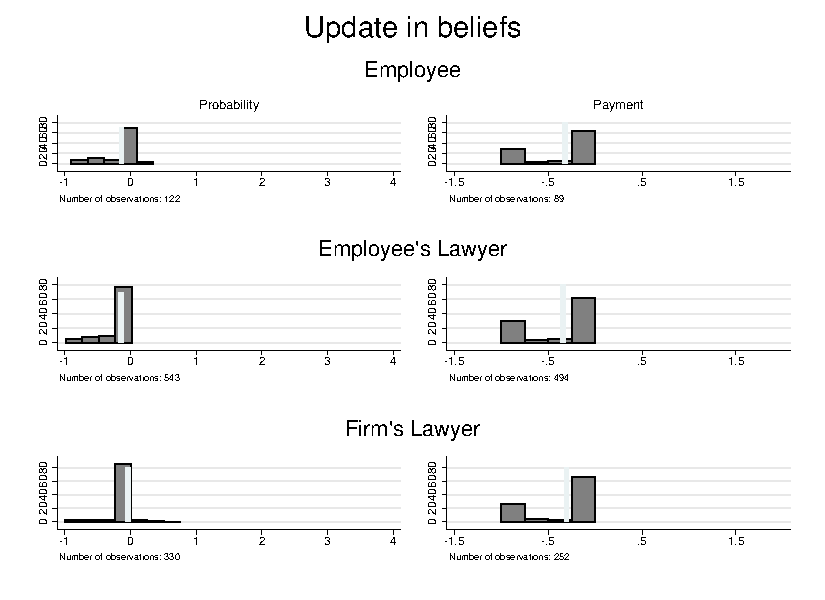
\includegraphics[width=\textwidth]{./Figures/update_belief.pdf}
\end{center}
{\footnotesize \textit{The histograms measures the update in relative terms. Width of bins is 0.25 }}
\end{figure}

\pagebreak

Now we test difference in initial and exit survey in expectations. The following table shows the results.

\begin{center}
\scriptsize{% Table generated by Excel2LaTeX from sheet 'ttest'
\begin{tabular}{rrrr}
\toprule
      & \multicolumn{1}{c}{Initial} & \multicolumn{1}{c}{Exit} & \multicolumn{1}{c}{p-value} \\
\midrule
\multicolumn{4}{c}{Probability} \\
\midrule
\midrule
Employee  & \multicolumn{1}{l}{79.927} & \multicolumn{1}{l}{71.945} & \multicolumn{1}{l}{0} \\
      & \multicolumn{1}{l}{(24.703)} & \multicolumn{1}{l}{(28.661)} & \multicolumn{1}{l}{} \\
Employees Lawyer & \multicolumn{1}{l}{77.007} & \multicolumn{1}{l}{67.658} & \multicolumn{1}{l}{0} \\
      & \multicolumn{1}{l}{(20.208)} & \multicolumn{1}{l}{(24.383)} & \multicolumn{1}{l}{} \\
Firms Lawyer & \multicolumn{1}{l}{40.822} & \multicolumn{1}{l}{42.267} & \multicolumn{1}{l}{0.122} \\
      & \multicolumn{1}{l}{(23.101)} & \multicolumn{1}{l}{(23.24)} & \multicolumn{1}{l}{} \\
      \midrule
\multicolumn{4}{c}{Payment levels} \\
\midrule
\midrule
Employee  & \multicolumn{1}{l}{54344.478} & \multicolumn{1}{l}{54930.941} & \multicolumn{1}{l}{0.804} \\
      & \multicolumn{1}{l}{(64865.672)} & \multicolumn{1}{l}{(66475.18)} & \multicolumn{1}{l}{} \\
Employees Lawyer & \multicolumn{1}{l}{97829.594} & \multicolumn{1}{l}{88209.612} & \multicolumn{1}{l}{0} \\
      & \multicolumn{1}{l}{(108525.677)} & \multicolumn{1}{l}{(97808.871)} & \multicolumn{1}{l}{} \\
Firms Lawyer & \multicolumn{1}{l}{56229.145} & \multicolumn{1}{l}{54309.441} & \multicolumn{1}{l}{0.564} \\
      & \multicolumn{1}{l}{(74573.935)} & \multicolumn{1}{l}{(67685.482)} & \multicolumn{1}{l}{} \\
      \midrule
\multicolumn{4}{c}{Payment logs} \\
\midrule
\midrule
Employee  & \multicolumn{1}{l}{10.219} & \multicolumn{1}{l}{10.269} & \multicolumn{1}{l}{0.454} \\
      & \multicolumn{1}{l}{(1.709)} & \multicolumn{1}{l}{(1.617)} & \multicolumn{1}{l}{} \\
Employees Lawyer & \multicolumn{1}{l}{10.855} & \multicolumn{1}{l}{10.771} & \multicolumn{1}{l}{0.002} \\
      & \multicolumn{1}{l}{(1.569)} & \multicolumn{1}{l}{(1.523)} & \multicolumn{1}{l}{} \\
Firms Lawyer & \multicolumn{1}{l}{9.422} & \multicolumn{1}{l}{9.483} & \multicolumn{1}{l}{0.554} \\
      & \multicolumn{1}{l}{(3.303)} & \multicolumn{1}{l}{(3.117)} & \multicolumn{1}{l}{} \\
\bottomrule
\end{tabular}%
}
\end{center}


\pagebreak

\subsection*{Treatments: Calculadora}

The following variables are dummies whether plaintiff and defendant (resp.) took part of the \emph{calculadora}.\\

\begin{center}
\scriptsize{
\begin{table}[htbp]\centering
\caption{\label{calcu_p_actora_by_calcu_p_dem} 
\textbf{Calculadora Actora by Calculadora Demandado}}
\begin{tabular} {@{} l r  r r @{}} \\ \hline
& \multicolumn{3}{@{} c @{}}{\textbf{Calculadora Demandado}} \\
\textbf{Calculadora Actora} & 
No &Yes &Total \\  \hline
No&    1,344&      214&    1,558\\
Yes&      867&      689&    1,556\\
Total&    2,211&      903&    3,114\\\hline 
\multicolumn{4}{@{}l}{\footnotesize{}}
\end{tabular}
\end{table}



}
\end{center}

\pagebreak

Take up treatment regression:

\begin{center}
\scriptsize{% Table generated by Excel2LaTeX from sheet 'Take_up'
\begin{tabular}{rrrrr}
\toprule
      & \multicolumn{2}{c}{Calculator} & \multicolumn{2}{c}{Survey} \\
\midrule
      & \multicolumn{1}{c}{Plaintiff} & \multicolumn{1}{c}{Defendant} & \multicolumn{1}{c}{Plaintiff} & \multicolumn{1}{c}{Defendant} \\
      &       &       &       &  \\
Female & \multicolumn{1}{l}{-0.0232} & \multicolumn{1}{l}{0.00164} & \multicolumn{1}{l}{-0.0178} & \multicolumn{1}{l}{-0.0154} \\
      & \multicolumn{1}{l}{(0.0210)} & \multicolumn{1}{l}{(0.0219)} & \multicolumn{1}{l}{(0.0233)} & \multicolumn{1}{l}{(0.0219)} \\
c\_antiguedad & \multicolumn{1}{l}{-0.00108} & \multicolumn{1}{l}{0.00266} & \multicolumn{1}{l}{-0.00244} & \multicolumn{1}{l}{0.000392} \\
      & \multicolumn{1}{l}{(0.00191)} & \multicolumn{1}{l}{(0.00197)} & \multicolumn{1}{l}{(0.00206)} & \multicolumn{1}{l}{(0.00195)} \\
c\_indem & \multicolumn{1}{l}{-0.000000141} & \multicolumn{1}{l}{-4.80e-08} & \multicolumn{1}{l}{-0.000000143} & \multicolumn{1}{l}{-8.74e-08} \\
      & \multicolumn{1}{l}{(0.000000131)} & \multicolumn{1}{l}{(0.000000131)} & \multicolumn{1}{l}{(0.000000152)} & \multicolumn{1}{l}{(0.000000145)} \\
dummy\_reinst & \multicolumn{1}{l}{0.00179} & \multicolumn{1}{l}{0.0162} & \multicolumn{1}{l}{0.0150} & \multicolumn{1}{l}{0.0439*} \\
      & \multicolumn{1}{l}{(0.0218)} & \multicolumn{1}{l}{(0.0227)} & \multicolumn{1}{l}{(0.0241)} & \multicolumn{1}{l}{(0.0228)} \\
Public Lawyer & \multicolumn{1}{l}{0.00118} & \multicolumn{1}{l}{0.00459} & \multicolumn{1}{l}{-0.0436*} & \multicolumn{1}{l}{-0.0117} \\
      & \multicolumn{1}{l}{(0.0211)} & \multicolumn{1}{l}{(0.0222)} & \multicolumn{1}{l}{(0.0240)} & \multicolumn{1}{l}{(0.0213)} \\
Constant  & \multicolumn{1}{l}{0.696***} & \multicolumn{1}{l}{0.378***} & \multicolumn{1}{l}{0.638***} & \multicolumn{1}{l}{0.310***} \\
      & \multicolumn{1}{l}{(0.0332)} & \multicolumn{1}{l}{(0.0349)} & \multicolumn{1}{l}{(0.0378)} & \multicolumn{1}{l}{(0.0341)} \\
      & \multicolumn{1}{l}{} & \multicolumn{1}{l}{} & \multicolumn{1}{l}{} & \multicolumn{1}{l}{} \\
Observations & \multicolumn{1}{l}{2066} & \multicolumn{1}{l}{2066} & \multicolumn{1}{l}{1862} & \multicolumn{1}{l}{1830} \\
R-squared & \multicolumn{1}{l}{0.00125} & \multicolumn{1}{l}{0.00120} & \multicolumn{1}{l}{0.00346} & \multicolumn{1}{l}{0.00286} \\
Dep Var Mean & \multicolumn{1}{l}{0.676} & \multicolumn{1}{l}{0.399} & \multicolumn{1}{l}{0.570} & \multicolumn{1}{l}{0.308} \\
\bottomrule
\end{tabular}%
}
\end{center}

\pagebreak



\subsection*{Conciliation (Convenio) in the day of treatment}

The main variable is convenio, a dummy variable indicating whether the parts conciled or not.\\

\begin{center}
\scriptsize{
\begin{table}[htbp]\centering
\caption{\label{convenio_by_calcu_p_actora} 
\textbf{Convenio by Calculadora Actora}}
\begin{tabular} {@{} l r  r r @{}} \\ \hline
& \multicolumn{3}{@{} c @{}}{\textbf{Calculadora Actora}} \\
\textbf{Convenio} & 
No &Yes &Total \\  \hline
No concilio&    1,405&    1,338&    2,743\\
Concilio&      153&      218&      371\\
Total&    1,558&    1,556&    3,114\\\hline 
\multicolumn{4}{@{}l}{\footnotesize{}}
\end{tabular}
\end{table}



}
\end{center}

\begin{center}
\scriptsize{
\begin{table}[htbp]\centering
\caption{\label{convenio_by_calcu_p_dem} 
\textbf{Convenio by Calculadora Demandado}}
\begin{tabular} {@{} l r  r r @{}} \\ \hline
& \multicolumn{3}{@{} c @{}}{\textbf{Calculadora Demandado}} \\
\textbf{Convenio} & 
No &Yes &Total \\  \hline
No concilio&    1,441&      480&    1,921\\
Concilio&      130&      132&      262\\
Total&    1,571&      612&    2,183\\\hline 
\multicolumn{4}{@{}l}{\footnotesize{}}
\end{tabular}
\end{table}



}
\end{center}


\vspace{5mm}


\pagebreak


\vspace{5mm}

\section{\Huge{Regression: Treatment effects}}



The following regressions has as dependent variable \emph{\textbf{convenio}}.\\



\subsection*{Simple regression (Correlation)}

\begin{table}[H]\centering \caption{Regression with \emph{calculadora} and controlling by junta.}
\begin{center}
\scriptsize{% Table generated by Excel2LaTeX from sheet 'Simple_regression'
\begin{tabular}{rrrrrrr}
\toprule
      & \multicolumn{1}{c}{(1)} & \multicolumn{1}{c}{(2)} & \multicolumn{1}{c}{(3)} & \multicolumn{1}{c}{(4)} & \multicolumn{1}{c}{(5)} & \multicolumn{1}{c}{(6)} \\
\midrule
      &       &       &       &       &       &  \\
Calculator plaintiff & 0.0419*** & 0.0374*** &       &       & -0.000788 & -0.00204 \\
      & (0.0116) & (0.0117) &       &       & (0.0115) & (0.0116) \\
Calculator defendant &       &       & 0.139*** & 0.130*** & 0.140*** & 0.130*** \\
      &       &       & (0.0149) & (0.0148) & (0.0153) & (0.0152) \\
Court 7 &       & 0.0247 &       & 0.0246 &       & 0.0245 \\
      &       & (0.0168) &       & (0.0165) &       & (0.0165) \\
Court 9 &       & 0.00772 &       & 0.00776 &       & 0.00764 \\
      &       & (0.0158) &       & (0.0155) &       & (0.0156) \\
Court 11 &       & 0.142*** &       & 0.132*** &       & 0.132*** \\
      &       & (0.0195) &       & (0.0193) &       & (0.0193) \\
Court 16 &       & -0.00898 &       & -0.00642 &       & -0.00681 \\
      &       & (0.0163) &       & (0.0155) &       & (0.0159) \\
Constant & 0.0982*** & 0.0640*** & 0.0787*** & 0.0468*** & 0.0790*** & 0.0477*** \\
      & (0.00754) & (0.0129) & (0.00573) & (0.0110) & (0.00750) & (0.0127) \\
      &       &       &       &       &       &  \\
Observations & 3114  & 3114  & 3114  & 3114  & 3114  & 3114 \\
R-squared & 0.00418 & 0.0351 & 0.0382 & 0.0646 & 0.0382 & 0.0646 \\
\bottomrule
\end{tabular}%
}
\end{center}
\end{table}

\subsection*{Conditioning...}

\begin{table}[H]\centering \caption{\emph{Calculadora actor}}
\begin{center}
\scriptsize{% Table generated by Excel2LaTeX from sheet 'Notification_actor'
\begin{tabular}{rrrrrrr}
\toprule
\multicolumn{1}{c}{} & \multicolumn{1}{c}{(1)} & \multicolumn{1}{c}{(2)} & \multicolumn{1}{c}{(3)} & \multicolumn{1}{c}{(4)} & \multicolumn{1}{c}{(5)} & \multicolumn{1}{c}{(6)} \\
\midrule
      &       &       &       &       &       &  \\
Calculator plaintiff & 0.0524** & 0.0319* & 0.0284*** & 0.0510* & 0.0301 & 0.0261** \\
      & (0.0222) & (0.0173) & (0.00949) & (0.0294) & (0.0223) & (0.0108) \\
Court 7 & 0.0112 & 0.0284 & 0.00678 & -0.000132 & 0.0287 & 0.00911 \\
      & (0.0343) & (0.0291) & (0.0124) & (0.0404) & (0.0335) & (0.0151) \\
Court 9 & -0.00703 & 0.00697 & 0.00398 & -0.0105 & 0.0120 & 0.0104 \\
      & (0.0333) & (0.0283) & (0.0116) & (0.0387) & (0.0320) & (0.0147) \\
Court 11 & 0.177*** & 0.0787*** & 0.128 & 0.188*** & 0.0821*** & 0.231 \\
      & (0.0359) & (0.0261) & (0.0927) & (0.0428) & (0.0298) & (0.152) \\
Court 16 & -0.0311 & -0.0403 & -0.00314 & -0.00784 & -0.00431 & 0.000650 \\
      & (0.0322) & (0.0271) & (0.0116) & (0.0426) & (0.0357) & (0.0174) \\
Constant  & 0.132*** & 0.131*** & 0.00424 & 0.133*** & 0.129*** & 0.00311 \\
      & (0.0268) & (0.0227) & (0.00976) & (0.0350) & (0.0277) & (0.0123) \\
      &       &       &       &       &       &  \\
Observations & 1285  & 1991  & 1123  & 890   & 1427  & 778 \\
R-squared & 0.0461 & 0.0150 & 0.0193 & 0.0446 & 0.00958 & 0.0249 \\
Conditioning on:   & Notification & Partial & No    & Notification \&  & Partial \&  & No Not \& \\
      &       & Notification & Notification & ITT   & ITT   & ITT \\
\bottomrule
\end{tabular}%
}
\end{center}
\end{table}

\begin{table}[H]\centering \caption{\emph{Calculadora demandado}}
\begin{center}
\scriptsize{% Table generated by Excel2LaTeX from sheet 'Notification_dem'
\begin{tabular}{rrrrrrr}
\toprule
\multicolumn{1}{c}{} & \multicolumn{1}{c}{(1)} & \multicolumn{1}{c}{(2)} & \multicolumn{1}{c}{(3)} & \multicolumn{1}{c}{(4)} & \multicolumn{1}{c}{(5)} & \multicolumn{1}{c}{(6)} \\
\midrule
      &       &       &       &       &       &  \\
Calculator defendant & \multicolumn{1}{l}{0.0727***} & \multicolumn{1}{l}{0.0991***} & \multicolumn{1}{l}{0.0941***} & \multicolumn{1}{l}{0.0788***} & \multicolumn{1}{l}{0.119***} & \multicolumn{1}{l}{0.0965***} \\
      & \multicolumn{1}{l}{(0.0224)} & \multicolumn{1}{l}{(0.0180)} & \multicolumn{1}{l}{(0.0308)} & \multicolumn{1}{l}{(0.0267)} & \multicolumn{1}{l}{(0.0201)} & \multicolumn{1}{l}{(0.0321)} \\
Court 7 & \multicolumn{1}{l}{0.0107} & \multicolumn{1}{l}{0.0306} & \multicolumn{1}{l}{0.00705} & \multicolumn{1}{l}{-0.00153} & \multicolumn{1}{l}{0.0280} & \multicolumn{1}{l}{0.0105} \\
      & \multicolumn{1}{l}{(0.0340)} & \multicolumn{1}{l}{(0.0289)} & \multicolumn{1}{l}{(0.0121)} & \multicolumn{1}{l}{(0.0399)} & \multicolumn{1}{l}{(0.0332)} & \multicolumn{1}{l}{(0.0149)} \\
Court 9 & \multicolumn{1}{l}{-0.00647} & \multicolumn{1}{l}{0.00799} & \multicolumn{1}{l}{0.00360} & \multicolumn{1}{l}{-0.00939} & \multicolumn{1}{l}{0.0139} & \multicolumn{1}{l}{0.0115} \\
      & \multicolumn{1}{l}{(0.0330)} & \multicolumn{1}{l}{(0.0281)} & \multicolumn{1}{l}{(0.0114)} & \multicolumn{1}{l}{(0.0382)} & \multicolumn{1}{l}{(0.0316)} & \multicolumn{1}{l}{(0.0146)} \\
Court 11 & \multicolumn{1}{l}{0.173***} & \multicolumn{1}{l}{0.0876***} & \multicolumn{1}{l}{0.128} & \multicolumn{1}{l}{0.182***} & \multicolumn{1}{l}{0.0938***} & \multicolumn{1}{l}{0.231} \\
      & \multicolumn{1}{l}{(0.0358)} & \multicolumn{1}{l}{(0.0258)} & \multicolumn{1}{l}{(0.0900)} & \multicolumn{1}{l}{(0.0429)} & \multicolumn{1}{l}{(0.0293)} & \multicolumn{1}{l}{(0.147)} \\
Court 16 & \multicolumn{1}{l}{-0.0326} & \multicolumn{1}{l}{-0.0324} & \multicolumn{1}{l}{-0.00164} & \multicolumn{1}{l}{-0.0136} & \multicolumn{1}{l}{-0.00798} & \multicolumn{1}{l}{0.00721} \\
      & \multicolumn{1}{l}{(0.0313)} & \multicolumn{1}{l}{(0.0264)} & \multicolumn{1}{l}{(0.0111)} & \multicolumn{1}{l}{(0.0424)} & \multicolumn{1}{l}{(0.0353)} & \multicolumn{1}{l}{(0.0172)} \\
Constant  & \multicolumn{1}{l}{0.127***} & \multicolumn{1}{l}{0.103***} & \multicolumn{1}{l}{0.00859} & \multicolumn{1}{l}{0.122***} & \multicolumn{1}{l}{0.0806***} & \multicolumn{1}{l}{0.00674} \\
      & \multicolumn{1}{l}{(0.0245)} & \multicolumn{1}{l}{(0.0211)} & \multicolumn{1}{l}{(0.00819)} & \multicolumn{1}{l}{(0.0290)} & \multicolumn{1}{l}{(0.0238)} & \multicolumn{1}{l}{(0.00946)} \\
      & \multicolumn{1}{l}{} & \multicolumn{1}{l}{} & \multicolumn{1}{l}{} & \multicolumn{1}{l}{} & \multicolumn{1}{l}{} & \multicolumn{1}{l}{} \\
Observations & \multicolumn{1}{l}{1285} & \multicolumn{1}{l}{1991} & \multicolumn{1}{l}{1123} & \multicolumn{1}{l}{890} & \multicolumn{1}{l}{1427} & \multicolumn{1}{l}{778} \\
R-squared & \multicolumn{1}{l}{0.0500} & \multicolumn{1}{l}{0.0295} & \multicolumn{1}{l}{0.0449} & \multicolumn{1}{l}{0.0500} & \multicolumn{1}{l}{0.0312} & \multicolumn{1}{l}{0.0565} \\
Conditioning on:   & \multicolumn{1}{l}{Notification} & \multicolumn{1}{l}{Partial} & \multicolumn{1}{l}{No  } & \multicolumn{1}{l}{Notification \& } & \multicolumn{1}{l}{Partial \& } & \multicolumn{1}{l}{No Not \&} \\
      & \multicolumn{1}{l}{} & \multicolumn{1}{l}{Notification} & \multicolumn{1}{l}{Notification} & \multicolumn{1}{l}{ITT} & \multicolumn{1}{l}{ITT} & \multicolumn{1}{l}{ITT} \\
\bottomrule
\end{tabular}%
}
\end{center}
\end{table}


\subsection*{Adding presence of employee}

\begin{table}[H]\centering \caption{Employee's presence}
\begin{center}
\scriptsize{% Table generated by Excel2LaTeX from sheet 'Presence_employee'
\begin{tabular}{rrrr}
\toprule
\multicolumn{1}{c}{} & \multicolumn{1}{c}{(1)} & \multicolumn{1}{c}{(2)} & \multicolumn{1}{c}{(3)} \\
\midrule
      &       &       &  \\
Calculator plaintiff & 0.0186* &       & -0.00951 \\
      & (0.0112) &       & (0.0111) \\
Calculator defendant &       & 0.0951*** & 0.0985*** \\
      &       & (0.0147) & (0.0149) \\
Employee present (EP) & 0.169*** & 0.115*** & 0.146*** \\
      & (0.0350) & (0.0232) & (0.0335) \\
Calculator plaintiff\#\#EP & 0.0356 &       & -0.0580 \\
      & (0.0445) &       & (0.0445) \\
Calculator defendant\#\#EP &       & 0.187*** & 0.209*** \\
      &       & (0.0460) & (0.0482) \\
Constant  & 0.0808*** & 0.0635*** & 0.0671*** \\
      & (0.00729) & (0.00557) & (0.00729) \\
      &       &       &  \\
Observations & 3114  & 3114  & 3114 \\
R-squared & 0.0485 & 0.0883 & 0.0897 \\
\bottomrule
\end{tabular}%
}
\end{center}
\end{table}

\subsection*{Instrumenting treatment with intent to treat}

...as treatment is endogenous with operation day.


\begin{table}[H]\centering \caption{IV (Second Stage). Plaintiff}
\begin{center}
\scriptsize{% Table generated by Excel2LaTeX from sheet 'IV'
\begin{tabular}{rrrrrrrr}
\toprule
      &       &       & \multicolumn{5}{c}{Actora} \\
\midrule
      & (1)   & (2)   & (3)   & (4)   & (5)   & (6)   & (7) \\
      &       &       &       &       &       &       &  \\
Dia tratamiento & 0.0336** & 0.0350** &       &       &       &       &  \\
      & (0.0133) & (0.0138) &       &       &       &       &  \\
      &       &       &       &       &       &       &  \\
Calculadora (instrumented with dia tratamiento) &       &       & 0.0485** & 0.0533*** & 0.0667* & 0.0545* & 0.0389*** \\
      &       &       & (0.0196) & (0.0199) & (0.0356) & (0.0296) & (0.0145) \\
      &       &       &       &       &       &       &  \\
junta\_2 &       & -0.00435 &       & 0.00704 & 0.0124 & 0.0182 & -0.00211 \\
      &       & (0.0181) &       & (0.0180) & (0.0362) & (0.0302) & (0.0136) \\
      &       &       &       &       &       &       &  \\
junta\_7 &       & 0.0382** &       & 0.0490*** & 0.0433 & 0.0791*** & 0.0117 \\
      &       & (0.0188) &       & (0.0186) & (0.0364) & (0.0306) & (0.0137) \\
      &       &       &       &       &       &       &  \\
junta\_9 &       & 0.0163 &       & 0.0280 & 0.0139 & 0.0487* & 0.00603 \\
      &       & (0.0177) &       & (0.0174) & (0.0346) & (0.0292) & (0.0124) \\
      &       &       &       &       &       &       &  \\
junta\_11 &       & 0.160*** &       & 0.162*** & 0.222*** & 0.153*** & 0.140 \\
      &       & (0.0218) &       & (0.0214) & (0.0379) & (0.0274) & (0.0978) \\
      &       &       &       &       &       &       &  \\
Notificado &       &       &       & 0.128*** & 0     & 0.0918*** & 0 \\
      &       &       &       & (0.0136) & (.)   & (0.0202) & (.) \\
      &       &       &       &       &       &       &  \\
Constant & 0.0994*** & 0.0531*** & 0.0998*** & -0.00738 & 0.102*** & 0.0184 & -0.000844 \\
      & (0.0107) & (0.0129) & (0.0110) & (0.0129) & (0.0254) & (0.0244) & (0.00770) \\
      &       &       &       &       &       &       &  \\
Observations & 2685  & 2685  & 2666  & 2666  & 1085  & 1690  & 976 \\
R-squared & 0.00215 & 0.0382 & 0.00325 & 0.0755 & 0.0519 & 0.0293 & 0.0236 \\
Conditioning on:  &       &       &       &       & Notificacion  & Not Parcial  & No Not  \\
\bottomrule
\end{tabular}%
}
\end{center}
\end{table}
\begin{table}[H]\centering \caption{IV (Second Stage). Defendant}
\begin{center}
\scriptsize{% Table generated by Excel2LaTeX from sheet 'IV'
\begin{tabular}{rrrrrr}
\toprule
\multicolumn{1}{c}{} & \multicolumn{5}{c}{Defendant} \\
\midrule
      & (3)   & (4)   & (5)   & (6)   & (7) \\
      &       &       &       &       &  \\
Calculator (instrumented with ITT) & 0.0973*** & 0.0875*** & 0.0766** & 0.0677** & 0.220*** \\
      & (0.0307) & (0.0306) & (0.0369) & (0.0338) & (0.0767) \\
Court 7 &       & 0.0245 & 0.0108 & 0.0356 & 0.0100 \\
      &       & (0.0163) & (0.0340) & (0.0290) & (0.0127) \\
Court 9 &       & 0.00891 & -0.00639 & 0.0119 & 0.00619 \\
      &       & (0.0154) & (0.0331) & (0.0282) & (0.0126) \\
Court 11 &       & 0.127*** & 0.173*** & 0.109*** & 0.133 \\
      &       & (0.0189) & (0.0357) & (0.0270) & (0.0855) \\
Court 16 &       & -0.0203 & -0.0321 & -0.0378 & 0.00867 \\
      &       & (0.0161) & (0.0319) & (0.0272) & (0.0131) \\
Notified &       & 0.105*** & 0     & 0.0843*** & 0 \\
      &       & (0.0149) & (.)   & (0.0188) & (.) \\
Constant & 0.0909*** & 0.0189 & 0.125*** & 0.0535* & -0.00627 \\
      & (0.0100) & (0.0123) & (0.0291) & (0.0274) & (0.0120) \\
      &       &       &       &       &  \\
Observations & 3114  & 3114  & 1285  & 1991  & 1123 \\
R-squared & 0.0347 & 0.0863 & 0.0500 & 0.0384 & . \\
Conditioning on:  &       &       & Notification & Partial Not & No Not  \\
\bottomrule
\end{tabular}%
}
\end{center}
\end{table}


\subsubsection*{First stage}


\begin{table}[H]\centering \caption{IV (First stage). Plaintiff}
\begin{center}
\scriptsize{% Table generated by Excel2LaTeX from sheet 'Firststage'
\begin{tabular}{rrrrrr}
\toprule
      & \multicolumn{5}{c}{Actora} \\
\midrule
      & \multicolumn{1}{c}{(3)} & \multicolumn{1}{c}{(4)} & \multicolumn{1}{c}{(5)} & \multicolumn{1}{c}{(6)} & \multicolumn{1}{c}{(7)} \\
\multicolumn{1}{l}{} & \multicolumn{1}{l}{} & \multicolumn{1}{l}{} & \multicolumn{1}{l}{} & \multicolumn{1}{l}{} & \multicolumn{1}{l}{} \\
\multicolumn{1}{l}{junta\_2} & \multicolumn{1}{l}{} & \multicolumn{1}{l}{0.0259} & \multicolumn{1}{l}{0.0279} & \multicolumn{1}{l}{0.0429} & \multicolumn{1}{l}{0.00500} \\
\multicolumn{1}{l}{} & \multicolumn{1}{l}{} & \multicolumn{1}{l}{(0.0253)} & \multicolumn{1}{l}{(0.0372)} & \multicolumn{1}{l}{(0.0336)} & \multicolumn{1}{l}{(0.0386)} \\
\multicolumn{1}{l}{} & \multicolumn{1}{l}{} & \multicolumn{1}{l}{} & \multicolumn{1}{l}{} & \multicolumn{1}{l}{} & \multicolumn{1}{l}{} \\
\multicolumn{1}{l}{junta\_7} & \multicolumn{1}{l}{} & \multicolumn{1}{l}{0.0146} & \multicolumn{1}{l}{0.0109} & \multicolumn{1}{l}{0.0363} & \multicolumn{1}{l}{-0.0141} \\
\multicolumn{1}{l}{} & \multicolumn{1}{l}{} & \multicolumn{1}{l}{(0.0235)} & \multicolumn{1}{l}{(0.0354)} & \multicolumn{1}{l}{(0.0309)} & \multicolumn{1}{l}{(0.0361)} \\
\multicolumn{1}{l}{} & \multicolumn{1}{l}{} & \multicolumn{1}{l}{} & \multicolumn{1}{l}{} & \multicolumn{1}{l}{} & \multicolumn{1}{l}{} \\
\multicolumn{1}{l}{junta\_9} & \multicolumn{1}{l}{} & \multicolumn{1}{l}{-0.0106} & \multicolumn{1}{l}{0.000000682} & \multicolumn{1}{l}{-0.0164} & \multicolumn{1}{l}{-0.0102} \\
\multicolumn{1}{l}{} & \multicolumn{1}{l}{} & \multicolumn{1}{l}{(0.0241)} & \multicolumn{1}{l}{(0.0366)} & \multicolumn{1}{l}{(0.0328)} & \multicolumn{1}{l}{(0.0357)} \\
\multicolumn{1}{l}{} & \multicolumn{1}{l}{} & \multicolumn{1}{l}{} & \multicolumn{1}{l}{} & \multicolumn{1}{l}{} & \multicolumn{1}{l}{} \\
\multicolumn{1}{l}{junta\_11} & \multicolumn{1}{l}{} & \multicolumn{1}{l}{0.000240} & \multicolumn{1}{l}{0.0108} & \multicolumn{1}{l}{0.0123} & \multicolumn{1}{l}{0.0165} \\
\multicolumn{1}{l}{} & \multicolumn{1}{l}{} & \multicolumn{1}{l}{(0.0231)} & \multicolumn{1}{l}{(0.0324)} & \multicolumn{1}{l}{(0.0276)} & \multicolumn{1}{l}{(0.0959)} \\
\multicolumn{1}{l}{} & \multicolumn{1}{l}{} & \multicolumn{1}{l}{} & \multicolumn{1}{l}{} & \multicolumn{1}{l}{} & \multicolumn{1}{l}{} \\
\multicolumn{1}{l}{Notificado} & \multicolumn{1}{l}{} & \multicolumn{1}{l}{0.0564***} & \multicolumn{1}{l}{0} & \multicolumn{1}{l}{0.0648***} & \multicolumn{1}{l}{0} \\
\multicolumn{1}{l}{} & \multicolumn{1}{l}{} & \multicolumn{1}{l}{(0.0153)} & \multicolumn{1}{l}{(.)} & \multicolumn{1}{l}{(0.0210)} & \multicolumn{1}{l}{(.)} \\
\multicolumn{1}{l}{} & \multicolumn{1}{l}{} & \multicolumn{1}{l}{} & \multicolumn{1}{l}{} & \multicolumn{1}{l}{} & \multicolumn{1}{l}{} \\
\multicolumn{1}{l}{dia\_tratamiento} & \multicolumn{1}{l}{0.682***} & \multicolumn{1}{l}{0.681***} & \multicolumn{1}{l}{0.727***} & \multicolumn{1}{l}{0.699***} & \multicolumn{1}{l}{0.654***} \\
\multicolumn{1}{l}{} & \multicolumn{1}{l}{(0.0112)} & \multicolumn{1}{l}{(0.0118)} & \multicolumn{1}{l}{(0.0178)} & \multicolumn{1}{l}{(0.0145)} & \multicolumn{1}{l}{(0.0205)} \\
\multicolumn{1}{l}{} & \multicolumn{1}{l}{} & \multicolumn{1}{l}{} & \multicolumn{1}{l}{} & \multicolumn{1}{l}{} & \multicolumn{1}{l}{} \\
\multicolumn{1}{l}{Constant} & \multicolumn{1}{l}{0.00911***} & \multicolumn{1}{l}{-0.0193} & \multicolumn{1}{l}{0.00103} & \multicolumn{1}{l}{-0.0490*} & \multicolumn{1}{l}{0.0158} \\
\multicolumn{1}{l}{} & \multicolumn{1}{l}{(0.00343)} & \multicolumn{1}{l}{(0.0156)} & \multicolumn{1}{l}{(0.0201)} & \multicolumn{1}{l}{(0.0251)} & \multicolumn{1}{l}{(0.0209)} \\
\multicolumn{1}{l}{} & \multicolumn{1}{l}{} & \multicolumn{1}{l}{} & \multicolumn{1}{l}{} & \multicolumn{1}{l}{} & \multicolumn{1}{l}{} \\
\multicolumn{1}{l}{Observations} & \multicolumn{1}{l}{2666} & \multicolumn{1}{l}{2666} & \multicolumn{1}{l}{1085} & \multicolumn{1}{l}{1690} & \multicolumn{1}{l}{976} \\
\multicolumn{1}{l}{R-squared} & \multicolumn{1}{l}{0.381} & \multicolumn{1}{l}{0.385} & \multicolumn{1}{l}{0.453} & \multicolumn{1}{l}{0.400} & \multicolumn{1}{l}{0.359} \\
\multicolumn{1}{l}{Conditioning on: } & \multicolumn{1}{l}{} & \multicolumn{1}{l}{} & \multicolumn{1}{l}{Notificacion } & \multicolumn{1}{l}{Not Parcial } & \multicolumn{1}{l}{No Not } \\
\bottomrule
\end{tabular}%
}
\end{center}
\end{table}
\begin{table}[H]\centering \caption{IV (First Stage). Defendant}
\begin{center}
\scriptsize{% Table generated by Excel2LaTeX from sheet 'Firststage'
\begin{tabular}{rrrrrr}
\toprule
\multicolumn{1}{c}{} & \multicolumn{5}{c}{Demandado} \\
\midrule
\multicolumn{1}{c}{} & \multicolumn{1}{c}{(3)} & \multicolumn{1}{c}{(4)} & \multicolumn{1}{c}{(5)} & \multicolumn{1}{c}{(6)} & \multicolumn{1}{c}{(7)} \\
\multicolumn{1}{l}{} & \multicolumn{1}{l}{} & \multicolumn{1}{l}{} & \multicolumn{1}{l}{} & \multicolumn{1}{l}{} &  \\
\multicolumn{1}{l}{junta\_2} & \multicolumn{1}{l}{} & \multicolumn{1}{l}{-0.00857} & \multicolumn{1}{l}{-0.0441} & \multicolumn{1}{l}{0.00521} & \multicolumn{1}{l}{0.0439*} \\
\multicolumn{1}{l}{} & \multicolumn{1}{l}{} & \multicolumn{1}{l}{(0.0251)} & \multicolumn{1}{l}{(0.0407)} & \multicolumn{1}{l}{(0.0365)} & \multicolumn{1}{l}{(0.0263)} \\
\multicolumn{1}{l}{} & \multicolumn{1}{l}{} & \multicolumn{1}{l}{} & \multicolumn{1}{l}{} & \multicolumn{1}{l}{} & \multicolumn{1}{l}{} \\
\multicolumn{1}{l}{junta\_7} & \multicolumn{1}{l}{} & \multicolumn{1}{l}{0.0251} & \multicolumn{1}{l}{0.0231} & \multicolumn{1}{l}{0.0604*} & \multicolumn{1}{l}{0.00956} \\
\multicolumn{1}{l}{} & \multicolumn{1}{l}{} & \multicolumn{1}{l}{(0.0232)} & \multicolumn{1}{l}{(0.0368)} & \multicolumn{1}{l}{(0.0326)} & \multicolumn{1}{l}{(0.0227)} \\
\multicolumn{1}{l}{} & \multicolumn{1}{l}{} & \multicolumn{1}{l}{} & \multicolumn{1}{l}{} & \multicolumn{1}{l}{} & \multicolumn{1}{l}{} \\
\multicolumn{1}{l}{junta\_9} & \multicolumn{1}{l}{} & \multicolumn{1}{l}{-0.00502} & \multicolumn{1}{l}{-0.0582} & \multicolumn{1}{l}{-0.0133} & \multicolumn{1}{l}{0.0336} \\
\multicolumn{1}{l}{} & \multicolumn{1}{l}{} & \multicolumn{1}{l}{(0.0236)} & \multicolumn{1}{l}{(0.0391)} & \multicolumn{1}{l}{(0.0344)} & \multicolumn{1}{l}{(0.0237)} \\
\multicolumn{1}{l}{} & \multicolumn{1}{l}{} & \multicolumn{1}{l}{} & \multicolumn{1}{l}{} & \multicolumn{1}{l}{} & \multicolumn{1}{l}{} \\
\multicolumn{1}{l}{junta\_11} & \multicolumn{1}{l}{} & \multicolumn{1}{l}{0.0433*} & \multicolumn{1}{l}{-0.00147} & \multicolumn{1}{l}{-0.0380} & \multicolumn{1}{l}{0.0288} \\
\multicolumn{1}{l}{} & \multicolumn{1}{l}{} & \multicolumn{1}{l}{(0.0232)} & \multicolumn{1}{l}{(0.0342)} & \multicolumn{1}{l}{(0.0288)} & \multicolumn{1}{l}{(0.0732)} \\
\multicolumn{1}{l}{} & \multicolumn{1}{l}{} & \multicolumn{1}{l}{} & \multicolumn{1}{l}{} & \multicolumn{1}{l}{} &  \\
\multicolumn{1}{l}{Notificado} & \multicolumn{1}{l}{} & \multicolumn{1}{l}{0.284***} & \multicolumn{1}{l}{0} & \multicolumn{1}{l}{0.158***} & \multicolumn{1}{l}{0} \\
\multicolumn{1}{l}{} & \multicolumn{1}{l}{} & \multicolumn{1}{l}{(0.0159)} & \multicolumn{1}{l}{(.)} & \multicolumn{1}{l}{(0.0224)} & \multicolumn{1}{l}{(.)} \\
\multicolumn{1}{l}{} & \multicolumn{1}{l}{} & \multicolumn{1}{l}{} & \multicolumn{1}{l}{} & \multicolumn{1}{l}{} &  \\
\multicolumn{1}{l}{dia\_tratamiento} & \multicolumn{1}{l}{0.395***} & \multicolumn{1}{l}{0.406***} & \multicolumn{1}{l}{0.647***} & \multicolumn{1}{l}{0.564***} & \multicolumn{1}{l}{0.104***} \\
\multicolumn{1}{l}{} & \multicolumn{1}{l}{(0.0118)} & \multicolumn{1}{l}{(0.0127)} & \multicolumn{1}{l}{(0.0189)} & \multicolumn{1}{l}{(0.0156)} & \multicolumn{1}{l}{(0.0145)} \\
\multicolumn{1}{l}{} & \multicolumn{1}{l}{} & \multicolumn{1}{l}{} & \multicolumn{1}{l}{} & \multicolumn{1}{l}{} &  \\
\multicolumn{1}{l}{Constant} & \multicolumn{1}{l}{0.00911***} & \multicolumn{1}{l}{-0.127***} & \multicolumn{1}{l}{0.0183} & \multicolumn{1}{l}{-0.0977***} & \multicolumn{1}{l}{-0.00791} \\
\multicolumn{1}{l}{} & \multicolumn{1}{l}{(0.00343)} & \multicolumn{1}{l}{(0.0161)} & \multicolumn{1}{l}{(0.0210)} & \multicolumn{1}{l}{(0.0266)} & \multicolumn{1}{l}{(0.0132)} \\
\multicolumn{1}{l}{} & \multicolumn{1}{l}{} & \multicolumn{1}{l}{} & \multicolumn{1}{l}{} & \multicolumn{1}{l}{} &  \\
\multicolumn{1}{l}{Observations} & \multicolumn{1}{l}{2656} & \multicolumn{1}{l}{2656} & \multicolumn{1}{l}{1088} & \multicolumn{1}{l}{1692} & \multicolumn{1}{l}{964} \\
\multicolumn{1}{l}{R-squared} & \multicolumn{1}{l}{0.156} & \multicolumn{1}{l}{0.254} & \multicolumn{1}{l}{0.352} & \multicolumn{1}{l}{0.289} & \multicolumn{1}{l}{0.0361} \\
\multicolumn{1}{l}{Conditioning on: } & \multicolumn{1}{l}{} & \multicolumn{1}{l}{} & \multicolumn{1}{l}{Notificacion } & \multicolumn{1}{l}{Not Parcial } & \multicolumn{1}{l}{No Not } \\
\bottomrule
\end{tabular}%
}
\end{center}
\end{table}


\subsection*{Controlling for number of cases (litigios) }



\begin{table}[H]\centering \caption{Number of cases}
\begin{center}
\scriptsize{% Table generated by Excel2LaTeX from sheet 'Num_litigios'
\begin{tabular}{rrrrrr}
\toprule
      & \multicolumn{1}{c}{(1)} & \multicolumn{1}{c}{(2)} & \multicolumn{1}{c}{(3)} & \multicolumn{1}{c}{(4)} & \multicolumn{1}{c}{(5)} \\
\midrule
      &       &       &       &       &  \\
Calculadora\_actor &       & -0.0495 &       & -0.0822 & -0.0725 \\
      &       & (0.0485) &       & (0.116) & (0.116) \\
      &       &       &       &       &  \\
Calculadora\_dem & 0.135*** &       & 0.158*** &       & 0.153** \\
      & (0.0456) &       & (0.0591) &       & (0.0595) \\
      &       &       &       &       &  \\
Litigios dem: 11-30 & 0.0649 &       & 0.191 & 0.188 & 0.188 \\
      & (0.0905) &       & (0.139) & (0.138) & (0.140) \\
      &       &       &       &       &  \\
Litigios dem: 31-100 & 0.0440 &       & 0.0513 & 0.0560 & 0.0520 \\
      & (0.0748) &       & (0.107) & (0.108) & (0.108) \\
      &       &       &       &       &  \\
Litigios dem: +100 & -0.0264 &       & -0.00986 & -0.0212 & -0.0157 \\
      & (0.0658) &       & (0.0948) & (0.0953) & (0.0951) \\
      &       &       &       &       &  \\
Litigios actor: 11-30 &       & -0.0191 & 0.0232 & 0.0266 & 0.0287 \\
      &       & (0.0454) & (0.109) & (0.111) & (0.110) \\
      &       &       &       &       &  \\
Litigios actor: 31-100 &       & -0.0212 & -0.0249 & -0.0181 & -0.0250 \\
      &       & (0.0406) & (0.0935) & (0.0939) & (0.0944) \\
      &       &       &       &       &  \\
Litigios actor: +100 &       & 0.0170 & -0.00373 & 0.00485 & 0.00313 \\
      &       & (0.0388) & (0.0859) & (0.0886) & (0.0881) \\
      &       &       &       &       &  \\
Constant & 0.0769 & 0.172*** & 0.0537 & 0.279* & 0.126 \\
      & (0.0751) & (0.0557) & (0.134) & (0.164) & (0.171) \\
      &       &       &       &       &  \\
Observations & 523   & 858   & 282   & 281   & 281 \\
R-squared & 0.0155 & 0.00424 & 0.0296 & 0.0242 & 0.0318 \\
\bottomrule
\end{tabular}%
}
\end{center}
\end{table}


\pagebreak


\subsection*{Update in beliefs}



\begin{table}[H]\centering \caption{Update in probability}
\begin{center}
\scriptsize{% Table generated by Excel2LaTeX from sheet 'Update_beleifs_prob'
\begin{tabular}{rrrr}
\toprule
      & \multicolumn{3}{c}{Settlement} \\
\midrule
      & \multicolumn{1}{c}{(Employee)} & \multicolumn{1}{c}{(Employee's Lawyer)} & \multicolumn{1}{c}{(Firm's Lawyer)} \\
      & \multicolumn{1}{c}{} & \multicolumn{1}{c}{} & \multicolumn{1}{c}{} \\
Update prob & -0.0505 & 0.00193 & 0.0156 \\
      & (0.128) & (0.0576) & (0.106) \\
Constant  & 0.179*** & 0.125*** & 0.219*** \\
      & (0.0351) & (0.0151) & (0.0209) \\
      &       &       &  \\
Observations & 151   & 672   & 403 \\
R-squared & 0.00104 & 0.00000195 & 0.0000645 \\
IndVarMean & -0.130 & -0.139 & -0.0279 \\
\bottomrule
\end{tabular}%
}
\end{center}
\end{table}


\begin{table}[H]\centering \caption{Update in payment}
\begin{center}
\scriptsize{% Table generated by Excel2LaTeX from sheet 'Update_beleifs_pago'
\begin{tabular}{rrrr}
\toprule
      & \multicolumn{3}{c}{Convenio} \\
\midrule
      & \multicolumn{1}{c}{(Actor)} & \multicolumn{1}{c}{(Rep Actor)} & \multicolumn{1}{c}{(Rep Demandado)} \\
      & \multicolumn{1}{c}{} & \multicolumn{1}{c}{} & \multicolumn{1}{c}{} \\
Update pago & 0.246* & -0.123 & 0.0555 \\
      & (0.128) & (0.0849) & (0.0783) \\
      &       &       &  \\
Constant  & 0.217*** & 0.121*** & 0.214*** \\
      & (0.0406) & (0.0176) & (0.0272) \\
      &       &       &  \\
Observations & 112   & 446   & 265 \\
R-squared & 0.0145 & 0.00717 & 0.00177 \\
IndVarMean & -0.0492 & -0.110 & -0.122 \\
\bottomrule
\end{tabular}%
}
\end{center}
\end{table}


\subsection*{Which conciliator is better? }


\begin{table}[H]\centering \caption{Dummies by each conciliator}
\begin{center}
\scriptsize{% Table generated by Excel2LaTeX from sheet 'Conciliator'
\begin{tabular}{rrrrr}
\toprule
      & \multicolumn{2}{c}{Defendant} & \multicolumn{2}{c}{Plaintiff } \\
\midrule
      & \multicolumn{1}{c}{(1)} & \multicolumn{1}{c}{(2)} & \multicolumn{1}{c}{(1)} & \multicolumn{1}{c}{(2)} \\
      &       &       &       &  \\
Calculator & 0.146*** & 0.166*** & 0.0389*** & 0.0435 \\
      & (0.0154) & (0.0389) & (0.0147) & (0.0335) \\
ANA   & 0.0104 & 0.0248 & 0.0215 & 0.109 \\
      & (0.0351) & (0.0374) & (0.0355) & (0.0760) \\
LUCIA & -0.0127 & -0.0361* & 0.00549 & 0.0393 \\
      & (0.0347) & (0.0211) & (0.0362) & (0.0704) \\
JACQUIE & 0.0389 & 0.00568 & 0.0373 & 0.0832 \\
      & (0.0330) & (0.0221) & (0.0349) & (0.0782) \\
MARINA & -0.0484* & -0.0135 & -0.0617** & -0.0961 \\
      & (0.0294) & (0.0212) & (0.0307) & (0.0681) \\
KARINA & 0.115* & 0.127 & 0.117* & -0.0109 \\
      & (0.0664) & (0.0872) & (0.0664) & (0.107) \\
MARIBEL & 0.0655 & -0.0310 & 0.0787* & -0.0315 \\
      & (0.0447) & (0.0471) & (0.0462) & (0.0759) \\
DEYANIRA & 0.132*** & 0.0967 & 0.128** & 0.121 \\
      & (0.0507) & (0.0614) & (0.0516) & (0.0871) \\
GUSTAVO & 0     & 0     & 0     & 0 \\
      & (.)   & (.)   & (.)   & (.) \\
CORRAL & 0.0380 & 0.0564 & 0.0495 & 0.0611 \\
      & (0.0351) & (0.0414) & (0.0356) & (0.0632) \\
AGUSTIN & -0.0449 & -0.0352 & -0.0505 & -0.0173 \\
      & (0.0308) & (0.0284) & (0.0313) & (0.0526) \\
MARGARITA & 0.0587* & 0.0555* & 0.0646** & 0.0427 \\
      & (0.0314) & (0.0298) & (0.0318) & (0.0550) \\
LUPITA & -0.0157 & 0.00930 & -0.0202 & -0.0453 \\
      & (0.0269) & (0.0282) & (0.0272) & (0.0454) \\
ISAAC & 0.0140 & -0.0186 & 0.0152 & 0.0274 \\
      & (0.0296) & (0.0257) & (0.0308) & (0.0521) \\
HIGUERA & 0.00401 & 0.0285 & 0.00413 & 0.0452 \\
      & (0.0236) & (0.0236) & (0.0241) & (0.0432) \\
DOCTOR & -0.0184 & 0.00784 & -0.0107 & -0.0159 \\
      & (0.0302) & (0.0272) & (0.0309) & (0.0405) \\
CESAR & -0.0229 & -0.0300 & -0.0326 & -0.0425 \\
      & (0.0328) & (0.0263) & (0.0337) & (0.0384) \\
Constant  & 0.0573*** & 0.0496*** & 0.0874*** & 0.0831*** \\
      & (0.0160) & (0.0149) & (0.0189) & (0.0254) \\
      &       &       &       &  \\
Interaction Term & NO    & YES   & NO    & YES \\
Observations & 2205  & 2205  & 2205  & 2205 \\
R-squared & 0.0784 & 0.0869 & 0.0365 & 0.0415 \\
\bottomrule
\end{tabular}%
}
\end{center}
\end{table}

\begin{table}[H]\centering \caption{Interaction term}
\begin{center}
\scriptsize{% Table generated by Excel2LaTeX from sheet 'Conciliator'
\begin{tabular}{rrr}
\toprule
\multicolumn{1}{c}{Interaction Terms} & \multicolumn{1}{c}{Defendant} & \multicolumn{1}{c}{Plaintiff } \\
\midrule
      &       &  \\
Calculator\#ANA & -0.0313 & -0.121 \\
      & (0.0751) & (0.0854) \\
Calculator\#LUCIA & 0.0569 & -0.0453 \\
      & (0.0815) & (0.0830) \\
Calculator\#JACQUIE & 0.0802 & -0.0601 \\
      & (0.0782) & (0.0877) \\
Calculator\#MARINA & -0.0856 & 0.0477 \\
      & (0.0686) & (0.0769) \\
Calculator\#KARINA & -0.0344 & 0.164 \\
      & (0.133) & (0.134) \\
Calculator\#MARIBEL & 0.161* & 0.142 \\
      & (0.0853) & (0.0938) \\
Calculator\#DEYANIRA & 0.0703 & 0.00278 \\
      & (0.104) & (0.108) \\
Calculator\#CORRAL & -0.0316 & -0.00780 \\
      & (0.0720) & (0.0763) \\
Calculator\#AGUSTIN & -0.0246 & -0.0422 \\
      & (0.0724) & (0.0649) \\
Calculator\#MARGARITA & 0.00763 & 0.0275 \\
      & (0.0728) & (0.0669) \\
Calculator\#LUPITA & -0.0852 & 0.0349 \\
      & (0.0614) & (0.0574) \\
Calculator\#ISAAC & 0.0909 & -0.0145 \\
      & (0.0694) & (0.0649) \\
Calculator\#HIGUERA & -0.0624 & -0.0561 \\
      & (0.0528) & (0.0524) \\
Calculator\#DOCTOR & -0.0601 & 0.00915 \\
      & (0.0651) & (0.0576) \\
Calculator\#CESAR & 0.00838 & 0.0142 \\
      & (0.0739) & (0.0594) \\
\bottomrule
\end{tabular}%
}
\end{center}
\end{table}

\subsection*{Some last controls }


\begin{table}[H]\centering \caption{Covariates employee survey}
\begin{center}
\scriptsize{% Table generated by Excel2LaTeX from sheet 'SS_control_survey'
\begin{tabular}{rrrrrr}
\toprule
\multicolumn{1}{c}{Variable } & \multicolumn{1}{c}{Obs} & \multicolumn{1}{c}{Mean} & \multicolumn{1}{c}{Std. Dev.} & \multicolumn{1}{c}{Min} & \multicolumn{1}{c}{Max} \\
\midrule
Enojo &       &       &       &       &  \\
Mediano & 213   & 0.1737089 & 0.3797515 & 0     & 1 \\
Poco  & 213   & 0.0704225 & 0.2564605 & 0     & 1 \\
Nada  & 213   & 0.1596244 & 0.3671202 & 0     & 1 \\
      &       &       &       &       &  \\
      &       &       &       &       &  \\
Compra bienes & 207   & 0.0628019 & 0.2431945 & 0     & 1 \\
      &       &       &       &       &  \\
Estudios &       &       &       &       &  \\
Secundaria & 213   & 0.2723005 & 0.4461923 & 0     & 1 \\
Preparatoria & 213   & 0.286385 & 0.4531364 & 0     & 1 \\
Mas que prepa & 213   & 0.370892 & 0.4841815 & 0     & 1 \\
      &       &       &       &       &  \\
Trabaja & 206   & 0.4223301 & 0.4951338 & 0     & 1 \\
Busca trabajo & 201   & 0.5472637 & 0.499004 & 0     & 1 \\
\bottomrule
\end{tabular}%
}
\end{center}
\end{table}

\begin{table}[H]\centering \caption{Controlling for some answers in employee survey}
\begin{center}
\scriptsize{% Table generated by Excel2LaTeX from sheet 'Answers_employee'
\begin{tabular}{rrrr}
\toprule
      & \multicolumn{1}{c}{(1)} & \multicolumn{1}{c}{(2)} & \multicolumn{1}{c}{(3)} \\
\midrule
Calculator plaintiff & -0.0284 &       & -0.0599 \\
      & (0.118) &       & (0.112) \\
Calculator defendant &       & 0.173*** & 0.175*** \\
      &       & (0.0583) & (0.0584) \\
Anger: fairly & 0.0667 & 0.0910 & 0.0915 \\
      & (0.0726) & (0.0715) & (0.0718) \\
Anger: little & 0.134 & 0.128 & 0.126 \\
      & (0.119) & (0.115) & (0.112) \\
Anger: nothing & 0.201** & 0.218** & 0.215** \\
      & (0.0934) & (0.0876) & (0.0880) \\
Buys durable goods & -0.109 & -0.130 & -0.136 \\
      & (0.0949) & (0.0982) & (0.101) \\
Secondary & 0.150*** & 0.123** & 0.123** \\
      & (0.0522) & (0.0538) & (0.0543) \\
High School & 0.236*** & 0.209*** & 0.212*** \\
      & (0.0641) & (0.0642) & (0.0656) \\
+ High School & 0.152*** & 0.116** & 0.118** \\
      & (0.0508) & (0.0535) & (0.0547) \\
Works at the time & 0.0391 & 0.0329 & 0.0335 \\
      & (0.0738) & (0.0709) & (0.0712) \\
Looking for a job & 0.000235 & 0.00360 & 0.00415 \\
      & (0.0732) & (0.0690) & (0.0693) \\
Constant  & -0.0185 & -0.0826 & -0.0275 \\
      & (0.125) & (0.0685) & (0.118) \\
      &       &       &  \\
Observations & 221   & 221   & 221 \\
R-squared & 0.0667 & 0.112 & 0.113 \\
\bottomrule
\end{tabular}%
}
\end{center}
\end{table}


\vspace{5mm}

\begin{center}
\scriptsize{
\begin{table}[htbp]\centering \caption{Covariates iniciales \label{sumstat}}
\begin{tabular}{l c c c c c}\hline\hline
\multicolumn{1}{c}{\textbf{Variable}} & \textbf{Mean}
 & \textbf{Std. Dev.}& \textbf{Min.} &  \textbf{Max.} & \textbf{N}\\ \hline
gen & 0.446 & 0.497 & 0 & 1 & 2108\\
c\_antiguedad & 4.049 & 5.462 & 0.003 & 44.822 & 2108\\
c\_indem & 55236.205 & 79282.709 & 0 & 1364212.625 & 2108\\
reinst & 0.49 & 0.5 & 0 & 1 & 2108\\
tipo\_abogado\_ac & 1.144 & 0.516 & 1 & 3 & 2108\\
\hline\end{tabular}
\end{table}
}
\end{center}

\begin{table}[H]\centering \caption{Controlling for some initial variables}
\begin{center}
\scriptsize{% Table generated by Excel2LaTeX from sheet 'Control_iniciales'
\begin{tabular}{rrrr}
\toprule
\multicolumn{1}{c}{} & \multicolumn{1}{c}{(1)} & \multicolumn{1}{c}{(2)} & \multicolumn{1}{c}{(3)} \\
\midrule
      &       &       &  \\
Calculadora\_actor & 0.0343** &       & 0.0153 \\
      & (0.0166) &       & (0.0163) \\
      &       &       &  \\
Calculadora\_dem &       & 0.157*** & 0.158*** \\
      &       & (0.0173) & (0.0174) \\
      &       &       &  \\
dummy\_gen & 0.0184 & 0.0166 & 0.0152 \\
      & (0.0162) & (0.0159) & (0.0159) \\
      &       &       &  \\
c\_antiguedad & -0.00334*** & -0.00397*** & -0.00396*** \\
      & (0.00101) & (0.00102) & (0.00103) \\
      &       &       &  \\
c\_indem & -0.000000230*** & -0.000000215*** & -0.000000239** \\
      & (8.54e-08) & (8.28e-08) & (9.35e-08) \\
      &       &       &  \\
dummy\_reinst & -0.0318* & -0.0311* & -0.0299* \\
      & (0.0169) & (0.0165) & (0.0167) \\
      &       &       &  \\
tipo\_abogado\_ac & -0.0136 & -0.00968 & -0.0103 \\
      & (0.0164) & (0.0153) & (0.0153) \\
      &       &       &  \\
Constant  & 0.159*** & 0.117*** & 0.108*** \\
      & (0.0286) & (0.0254) & (0.0279) \\
      &       &       &  \\
Observations & 1812  & 1802  & 1794 \\
R-squared & 0.0125 & 0.0615 & 0.0634 \\
\bottomrule
\end{tabular}%
}
\end{center}
\end{table}

%%%%%%%%%%%%%%%%%%%%%%%%%%%%%%%%%%%%%%%%%%%%%%%%%%%%%%%%%%%%%%%%%%%%%%%%%%%%%%%%
\end{document}
